Comme nous l'illustrions dans l'état de l'art de cette thèse de
nombreuses implémentations des \emph{sous-ensembles flous spatialisés}
ont été proposées. On y retrouve aussi bien des approches vectorielles
\autocite{Kanjilal2010,Dilo2007,Zoghlami2016} ou raster
\autocite{Bloch1996}, que des approches fondées sur la sélection
d'objets préexistants \autocite{Duraciova2017}.

Chacune de ces solutions a des avantages et des inconvénients qu'il
est nécessaire d'étudier. De plus, toutes ses solutions ne permettent
pas nécessairement de conserver toutes les qualités du modèle
théorique. Par exemple, les approches vectorielles proposant une
discrétisation du sous-ensemble flou, comme celles proposées par
\textcite{Kanjilal2010,Zoghlami2016}, ont une précision de
représentation qui dépend du nombre de régions utilisées pour
discrétiser le \emph{sous-ensemble flou.} Si elles sont au nombre de
deux, ces implémentations se comportent comme les modèles
\enquote{exacts} et ne sont pas plus utilisables. L'augmentation du
nombre de vecteurs permet de régler ce problème et de représenter tout
type de \emph{zones de localisation.}


\tdi{OK : On veut un modèle qui permet de prendre en compte des relations
  de localisation traduisant des limites assez nettes (en dessous de)
  et des relations avec des limites très continues (proches [voir
  concept similaire dans l'ontologie]).}

\tdi{OK : Possibilité de construire des zones de localisation issues de
  relations de localisation non linéaire (en dessous de).}

Chacune de ces deux implémentations permet la construction de
\emph{zones de localisation compatibles} à partir de \emph{relations
  de localisation} non linéaires. En effet, bien qu'elles imposent
toutes deux un échantillonnage des sous-ensembles flous, elles
permettent de rendre des variations non linéaires.

De la même manière, ces deux approches permettent de construire des
\emph{zones de localisation} dont les limites peuvent être
\emph{imprécises} ou assez précises.


Nous proposons de confronter les deux implémentations qui nous
semblent être les plus prometteuses, l'utilisation \emph{d'alpha-cuts}
vectorielles et l'utilisation de rasters.

\subsection{Exemple comparatif}

Les implémentations de la \emph{théorie des sous-ensembles flous} à
l'aide d'une approche par \emph{alpha-cuts} ou par raster nous
semblent toutes les deux pertinentes pour notre cas
d'utilisation. Nous proposons donc de les appliquer à une même exemple
pour trancher en faveur de l'une ou de l'autre
\autocite{Bunel2019a}. Pour ce faire nous avons sélectionné un des
\emph{indices de localisation} du \emph{fil rouge} : \enquote{La
  victime est située sous une ligne électrique 3 brins}, qui présente
le double avantage d'être simple à modéliser ---~et donc à
comparer~---, tout en utilisation une \emph{relation de localisation,}
décomposable. Cet exemple nous permet donc de tester, en plus de la
modélisation des \emph{zones de localisation,} leur intersection.

% Décomposition de l'indice
La \emph{relation de localisation} que nous avons identifiée comme la
plus adaptée à la formalisation de cet \emph{indice de localisation}
est \onto[orl]{Sous\-Pro\-che\-De}, traduisant une relation sur l'axe
vertical (l'altitude du \emph{sujet} est plus basse que celle de
\emph{l'objet de référence}), contrainte par une distance
planimétrique (\autoref{anx:orl_dic}).

Ce concept nous semble plus pertinent que la \emph{relation}
englobante (\onto[orl]{Sous\-Altitude}) ou plus précise
(\onto[orl]{Sous\-Recouvert\-Par}) s'explique par la nécessité

Cette \emph{relation} se décompose en deux \emph{relations de
  localisation atomiques} :
\onto[orla]{Al\-ti\-tu\-de\-Stric\-te\-ment\-Inf\-érieu\-re} et
\onto[orla]{Dis\-tan\-ce\-Quan\-ti\-ta\-ti\-ve\-Pla\-ni\-mé\-tri\-que},
traduisant respectivement, la notion de position sur l'axe vertical et
la contrainte posée sur la distance planimétrique. Conformément au
\emph{principe de décomposition} et à notre méthodologie (Chapitres
\ref{chap:02} et \ref{chap:04}), la \emph{zone de localisation
  compatible} correspondant à la \emph{relation de localisation}
\onto[orl]{Sous\-Pro\-che\-De} peut être créée en intersectant les
deux \emph{zones de localisation compatibles} résultant de la
\emph{spatialisation} de ces deux \emph{relations de localisation
  atomiques.}

% Définition fonctions appartenance
La construction des \emph{zones de localisation compatibles}
correspondant à chacune des \emph{relations de localisation atomiques}
nécessite de définir des \emph{fonctions d'appartenance} ($f_A$), qui,
associent à chaque élément de l'ensemble traité, un degré ---~compris
entre 0 et 1~--- définissant l'appartenance de l'élément au
\emph{sous-ensemble flou} (Section \ref{subsec:theorie_flou}). Dans
notre contexte, où les \emph{sous-ensembles fous} représentent des
\emph{objets géographiques} et chaque élément une position, ces
fonctions définissent l'appartenance de chacune d'entre elles à la
\emph{zone de localisation compatible} construite. La définition des
\emph{fonctions d'appartenance} est donc une étape extrêmement
importante, puisqu'elle définit les règles de construction des
\emph{zones de localisation} et donc la sémantique des \emph{relations
  de localisation atomiques.}

Leur définition se fait en deux étapes,
tout d'abord il faut identifier une \emph{métrique,} c'est-à-dire une
valeur quantitative ou qualitative et calculable en chaque position 

et ensuite la \emph{fonction d'appartenance,} transformant les valeurs
de la \emph{métrique} en un \emph{degré d'appartenance.} Dans notre
exemple, les \emph{métriques} à utiliser sont assez instinctives et
simples à calculer. Par exemple, la \emph{relation de localisation
  atomique}
\onto[orla]{Dis\-tan\-ce\-Quan\-ti\-ta\-ti\-ve\-Pla\-ni\-mé\-tri\-que}
traduit le fait que la distance planimétrique entre le \emph{sujet} et
\emph{l'objet de référence} est faible. La métrique adaptée est donc
la distance euclidienne entre chaque position et le point le plus
proche de \emph{l'objet de référence} (\autoref{fig:ISO_DIST_HT}).

\begin{carte}
  \centering
  \begin{tikzpicture}
  \tikzset{et/.style={above,font=\footnotesize\vphantom{Ag}}}
  % 
  \node[inner sep=0pt, anchor=south west] (image) at (0,0){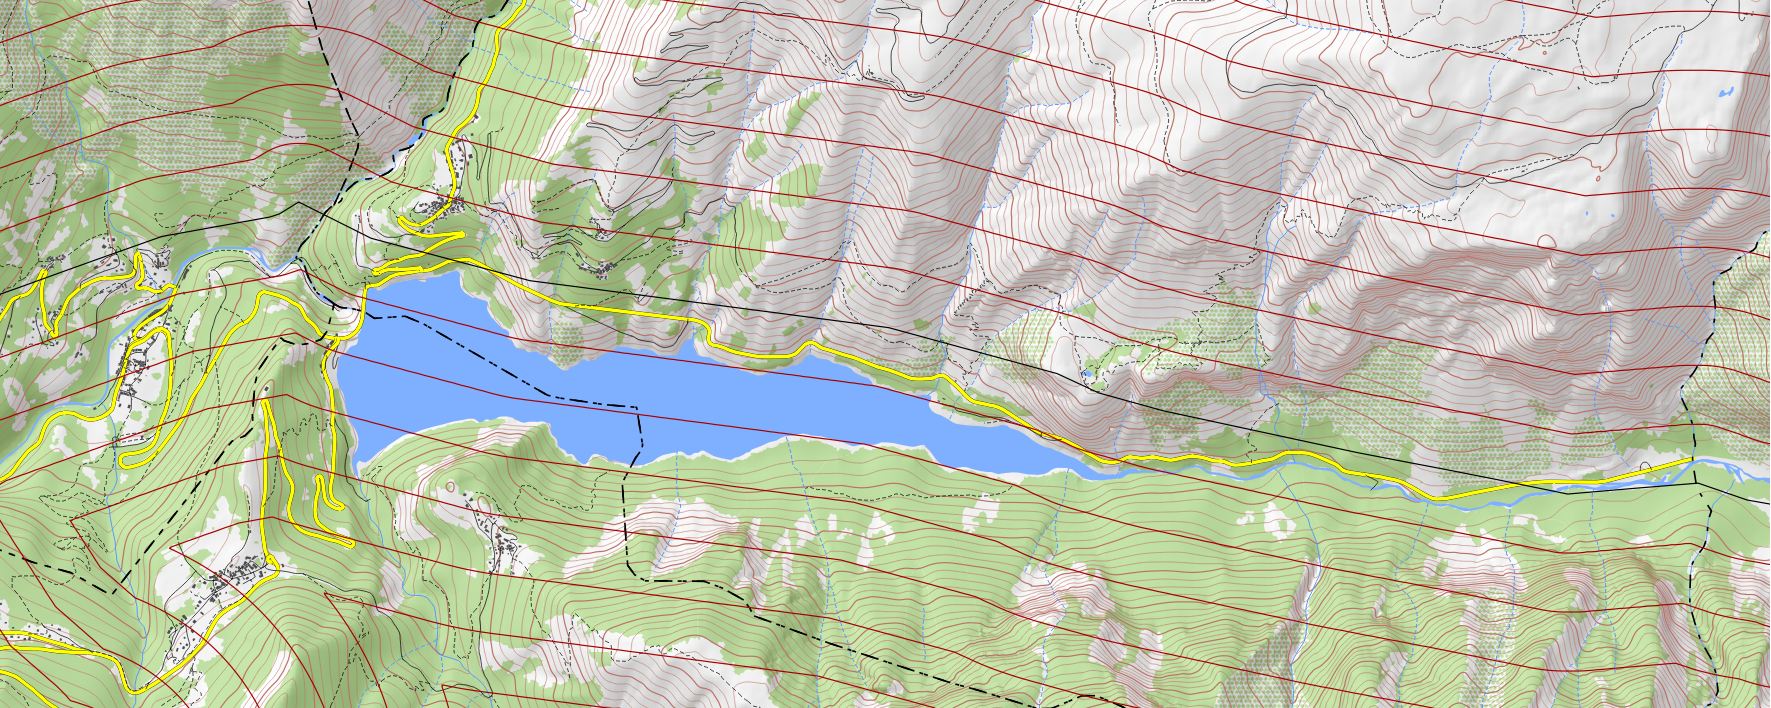
\includegraphics{./figures/Raster_ISO_DIST_HT.png}};
  % 
  \begin{scope}
    \node (P2) at ([yshift=-.5cm]image.south east) {};
    \node (P1) at ([yshift=-.5cm]image.south west) {};

    \node (rect) [anchor=north west, minimum width=1cm,minimum
    height=.25cm] at ([yshift=-.25cm]P1) {}; \path[draw=RdBu-9-1, line
    width=.4mm](rect.west) --([xshift=-1ex]rect.south) -- ([xshift=1ex]rect.north)
    -- (rect.east);
    \node[anchor=west, font=\tiny\vphantom{Ag}, text width = 4cm] at
    ([xshift=1ex]rect.east) {Ligne électrique utilisée comme
      \emph{objet de référence}};

    \node (rect2) [anchor=north west, minimum width=1cm,minimum
    height=.25cm] at ([xshift=5.5cm,yshift=-.25cm]P1) {};
    \path[draw=RdBu-9-9, line width=.25mm](rect2.west)
    --([xshift=-1ex]rect2.north) -- ([xshift=1ex]rect2.south) --
    (rect2.east); \node[anchor=west, font=\tiny\vphantom{Ag}, text
    width = 4cm] at ([xshift=1ex]rect2.east) {Isolignes d'éloignement
      à \emph{l'objet de référence} (équidistance \SI{250}{\meter})};

    % Échelle
    \draw[-] (P2 |- -1cm,-1cm) --++ (-1,0) node[et,pos=.5] {\SI{500}{\meter}};
    % Légende détaillée
    \path (P1) -- (P2) node[pos=.5, yshift=-1cm] {\tiny Pour la légende détaillée du fond topographique voir \autoref{anx:topo_leg}. Sources: BD TOPO 2018, BD ALTI 2018.}; 
  \end{scope}
\end{tikzpicture}
  \caption{\emph{Métrique} pour la \emph{relation de localisation
      atomique}
    \protect\onto[orla]{Dis\-tan\-ce\-Quan\-ti\-ta\-ti\-ve\-Pla\-ni\-mé\-tri\-que}
    : La distance planaire à la ligne électrique trois brins.}
  \label{fig:ISO_DIST_HT}
\end{carte}

La \emph{relation de localisation atomique}
\onto[orla]{Al\-ti\-tu\-de\-Stric\-te\-ment\-Inf\-érieu\-re} traduit,
quant à elle, un positionnement relatif sur l'axe vertical. La
\emph{métrique} la plus adaptée est donc la différence entre
l'altitude du point le plus proche de \emph{l'objet de référence} et
l'altitude de chaque position (\autoref{fig:ISO_DALT_HT}).

\begin{carte}
  \centering
  \begin{tikzpicture}
  \tikzset{et/.style={above,font=\footnotesize\vphantom{Ag}}}
  % 
  \node[inner sep=0pt, anchor=south west] (image) at (0,0){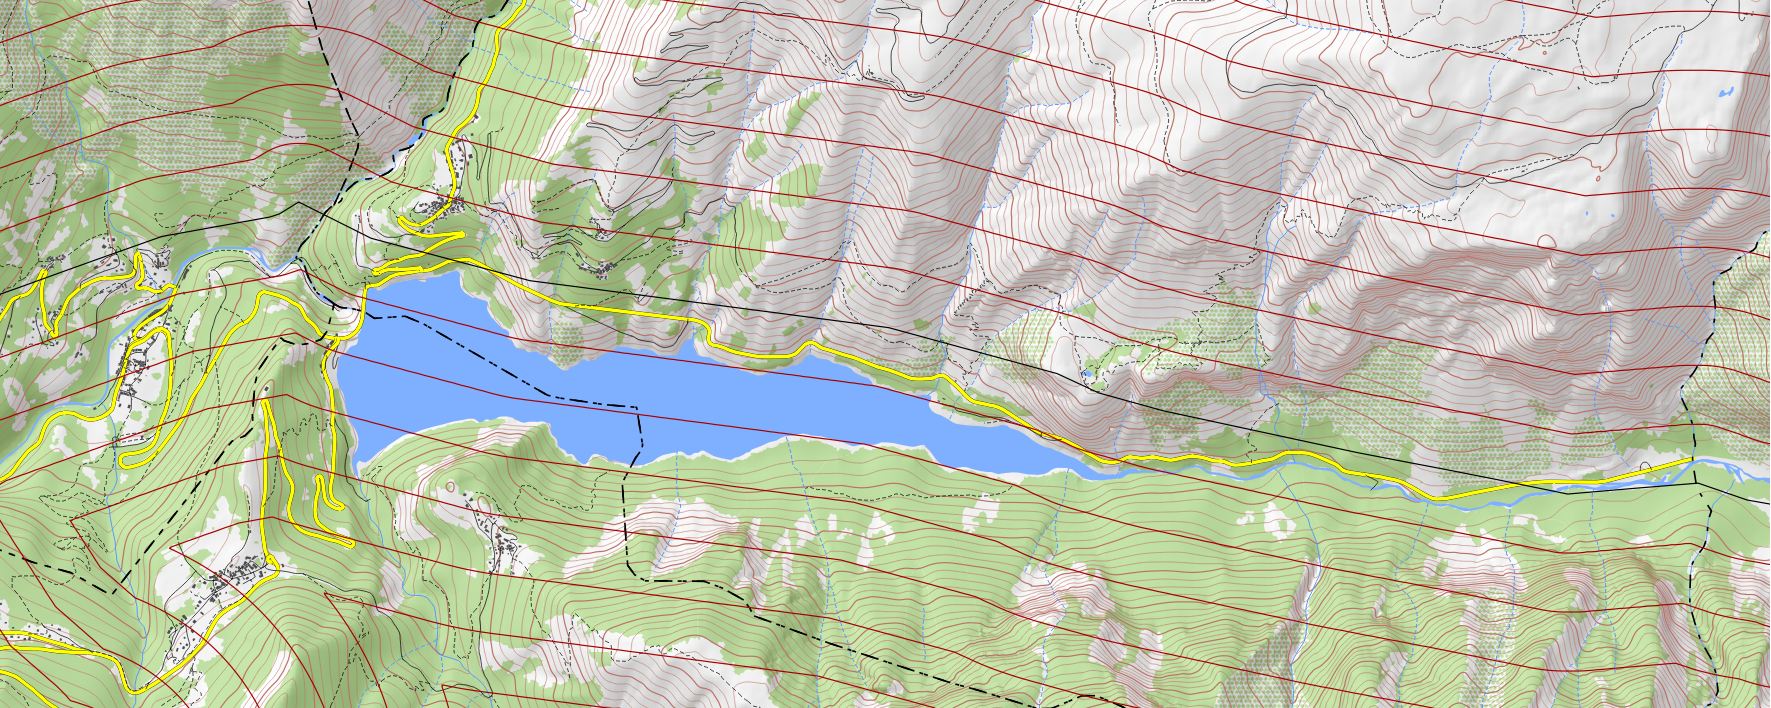
\includegraphics{./figures/Raster_ISO_DIST_HT.png}};
  % 
  \begin{scope}
    \node (P2) at ([yshift=-.5cm]image.south east) {};
    \node (P1) at ([yshift=-.5cm]image.south west) {};

    \node (rect) [anchor=north west, minimum width=1cm,minimum
    height=.25cm] at ([yshift=-.25cm]P1) {}; \path[draw=RdBu-9-1, line
    width=.4mm](rect.west) --([xshift=-1ex]rect.south) -- ([xshift=1ex]rect.north)
    -- (rect.east);
    \node[anchor=west, font=\tiny\vphantom{Ag}, text width = 4cm] at
    ([xshift=1ex]rect.east) {Ligne électrique utilisée comme
      \emph{objet de référence}};

    \node (rect2) [anchor=north west, minimum width=1cm,minimum
    height=.25cm] at ([xshift=5.5cm,yshift=-.25cm]P1) {};
    \path[draw=RdBu-9-9, line width=.25mm](rect2.west)
    --([xshift=-1ex]rect2.north) -- ([xshift=1ex]rect2.south) --
    (rect2.east); \node[anchor=west, font=\tiny\vphantom{Ag}, text
    width = 4cm] at ([xshift=1ex]rect2.east) {Isolignes d'éloignement
      à \emph{l'objet de référence} (équidistance \SI{250}{\meter})};

    % Échelle
    \draw[-] (P2 |- -1cm,-1cm) --++ (-1,0) node[et,pos=.5] {\SI{500}{\meter}};
    % Légende détaillée
    \path (P1) -- (P2) node[pos=.5, yshift=-1cm] {\tiny Pour la légende détaillée du fond topographique voir \autoref{anx:topo_leg}. Sources: BD TOPO 2018, BD ALTI 2018.}; 
  \end{scope}
\end{tikzpicture}
  \caption{Différence entre l'altitude locale et l'altitude de la
    ligne électrique la plus proche.}
  \label{fig:ISO_DALT_HT}
\end{carte}

La transformation des valeurs de ces deux métriques en degré
d'appartenance se fait à l'aide d'une fonction d'appartenance qu'il
convient de définir. Pour ce faire nous procédons généralement en deux
étapes. La première consiste à identifier la forme de \emph{la
  fonction d'appartenance} qui nous semble être la plus pertinente
pour retranscrire la sémantique de la \emph{relation de localisation
  atomique.} Puis nous identifions les seuils de cette
fonction. Ainsi, la première étape permet \footnote{Conjointement à la
  sélection d'une \emph{métrique.}} de fixer la sémantique de la
\emph{relation,} alors que la seconde étape fait plus office de
paramétrisation fine.

La \emph{relation de localisation atomique}
\onto[orla]{Dis\-tan\-ce\-Quan\-ti\-ta\-ti\-ve\-Pla\-ni\-mé\-tri\-que}
est utilisée pour figurer le fait que le \emph{sujet} n'est pas très
éloigné de \emph{l'objet de référence.} Ainsi, une position
\enquote{proche} de \emph{l'objet de référence} doit avoir un
\emph{degré d'appartenance} à la \emph{zone de localisation
  compatible} correspondant à cette \emph{relation de localisation
  atomique} plus élevé qu'une position qui en est éloigné. Le degré
d'appartenance doit donc diminuer lorsque la distance à \emph{l'objet
  de référence} (\ie la valeur de la métrique) augmente. La forme de
la fonction d'appartenance étant fixée, nous pouvons à présent en
définir les seuils. Deux valeurs sont à fixer, la première est la
distance à partir de laquelle le degré d'appartenance décroit. Si elle
est nulle le degré d’appartenance décroit dès que la distance
augmente, sinon il y aura une zone, dont la largeur dépend de la
valeur choisie, où le degré d'appartenance sera maximal. Définir ce
premier seuil revient à se demander quelle est la distance à partir de
laquelle on ne peut plus considérer que l'on est \enquote{proche}
d'une ligne électrique. Pour cet exemple nous avons fixé empiriquement
cette valeur à \SI{50}{\meter}. Le second seuil à fixer est la
distance à partir de laquelle le degré d'appartenance est nul. De
manière tout aussi empirique, nous avons fixé cette valeur à
\SI{100}{\meter}. Ainsi, entre 0 et 50 mètres, le degré d'appartenance
est de 1, puis il décroit jusqu’à être de 0 à 100 mètres et reste nul
au-delà, comme le montre la figure \ref{fig:fnc_app_Dist}.

La définition de la forme de la fonction d'appartenance pour la
\emph{relation de localisation atomique}
\onto[orla]{Al\-ti\-tu\-de\-Stric\-te\-ment\-Inf\-érieu\-re} ne pose
pas non plus de problèmes particuliers. Comme cette \emph{relation}
traduit une position relative sur l'axe vertical, le degré
d'appartenance doit être à 1 lorsque l'altitude de la position est
inférieure à celle de \emph{l'objet de référence} (\ie que la métrique
est négative) et nul dans le cas contraire (\ie que la métrique est
positive). Il faut alors définir les valeurs de la métrique à partir
desquelles le degré d'appartenance est de 1 ou de 0. Étant donné que
la différence d'altitude est calculée à partir du sommet de la ligne
électrique nous avons considéré que toute position dont l'altitude
était inférieure au point le plus proche de la ligne électrique (\ie
dès que la valeur de la métrique est négative) avait un degré
d'appartenance de 1. Nous avons fixé le second seuil à \SI{5}{\meter},
ce qui permet d'ajouter une petite marge d'erreur. Ainsi, le degré
d'appartenance est de 1 jusqu’à ce que la différence d'altitude soit
nulle, puis il décroit rapidement jusqu'a atteindre la valeur de 0
lorsque la différence est de \SI{5}{\meter} (\ie que la position est
\SI{5}{\meter} au-dessus du sommet de la ligne électrique), la valeur
reste nulle au-delà (Figure \ref{fig:fnc_app_AltInf}).

\begin{figure}
  \centering
  \subfloat{%
    \begin{tikzpicture}[scale=.7]
  \def\decalageX{-.2}
  \def\decalageY{-.2}
  % Courbe
  \begin{scope}[transparency group]
    % fond
    \begin{scope}
      \path[ffa] (0,2) -- (2.5,2) -- (5, 0)  -- (0,0) -- cycle;
    \end{scope}
    % bords
    \begin{scope}
      \path[ffc] (0,2) -- (2.5,2) -- (5, 0) -++ (3,0) ;
      \path[ffc_fade] (8,0) -- (9,0) ;
    \end{scope}
  \end{scope}
  % Axes X, Y
  \begin{scope}
    % Axe X
    \begin{scope}
      % Axe
      \draw[->] (0, \decalageX) --++ (9, 0) coordinate (x axis);
      % Graduations
      \foreach \n/\t in {0/{0},1/{20},2/{40},3/{60},4/{80},5/{100},6/{120},7/{140},8/{160}}
      {
        \draw[-] (\n, \decalageX - .05) --++ (0, .1);
        \node[below, font=\footnotesize] at (\n, \decalageX - .05) {\t};
      }
      % label
      \node[above left, yshift=.1cm, font=\small] at (x axis) {$Distance\ (m)$};
    \end{scope}
    % Axe Y
    \begin{scope}
      % Axe
      \draw[-] (\decalageY ,0) --++ (0, 2) coordinate (y axis);
      % Graduations
      \foreach \n/\t in {0/{0},2/{1}}
      {
        \draw[-] (\decalageY -.05, \n) --++ (.1, 0);
        \node[left, font=\footnotesize] at (\decalageY -.05, \n) {\t};
      }
      % Label
      \node[above] at (y axis) {$\mu$};
    \end{scope}
  \end{scope}
  \begin{scope}
    % Seuil 1
    \draw[ffc,line width=.5] (2.5,\decalageY) -- (2.5,2);
    \draw[fill, RdBu-9-1] (2.5,\decalageY) circle (2pt);
    \draw[fill, RdBu-9-1] (2.5,2) circle (2pt);
    % Seuil 2
    \draw[ffc,line width=.5] (5,\decalageY) -- (5,0);
    \draw[fill, RdBu-9-1] (5,\decalageY) circle (2pt);
    \draw[fill, RdBu-9-1] (5,0) circle (2pt);
  \end{scope}
\end{tikzpicture}

    \label{fig:fnc_app_Dist}
  }
  \hfill%
  \subfloat{%
    \begin{tikzpicture}[scale=.75]
  \def\decalageX{-.2}
  \def\decalageY{-.2}
  % Courbe
  \begin{scope}[transparency group]
    % fond
    \begin{scope}
      \draw[ffa] (1,2) -- (4.5, 2) -- (5.5,0) -- (1,0)-- cycle;
      \draw[ffa_fade_m] (0,2) -- (1, 2) -- (1,0) -- (0,0)-- cycle;
    \end{scope}
    % bords
    \begin{scope}
      \path[ffc] (1, 2) --(4.5, 2) -- (5.5,0) -- (8,0);
      \path[ffc_fade_m] (0,2) -- (1,2);
      \path[ffc_fade] (8,0) -- (9,0) ;
    \end{scope}
  \end{scope}
  % Axes
  \begin{scope}
    % Axe X
    \begin{scope}
      % Axe
      \draw[<->] (0, \decalageX) --++ (9, 0) coordinate (x axis);
      % Graduations
      \foreach \n/\t in {.5/{-20},1.5/{-15},2.5/{-10},3.5/{-5},4.5/{0},5.5/{5},6.5/{10},7.5/{15},8.5/{20}}
      {
        \draw[-] (\n, \decalageX - .05) --++ (0, .1);
        \node[below, font=\footnotesize] at (\n, \decalageX - .05) {\t};
      }
      % label
      \node[above left, yshift=.1cm, font=\small] at (x axis) {$\Delta\,Altitude\,(m)$};
    \end{scope}
    % Axe Y
    \begin{scope}
      % Axe
      \draw[-] (\decalageY ,0) --++ (0, 2) coordinate (y axis);
      % Graduations
      \foreach \n/\t in {0/{0},2/{1}}
      {
        \draw[-] (\decalageY -.05, \n) --++ (.1, 0);
        \node[left, font=\footnotesize] at (\decalageY -.05, \n) {\t};
      }
      % Label
      \node[above] at (y axis) {$\mu$};
    \end{scope}
  \end{scope}
  % Analyse
  \begin{scope}
    \draw (4.5,0) -- (4.5,2);
    \draw[fill] (4.5,0) circle (1pt);
    \draw[fill] (4.5,2) circle (1pt);
    \node[above] at (4.5,2) {P};
  \end{scope}
\end{tikzpicture}

    \label{fig:fnc_app_AltInf}
  }
  \caption{Fonctions d'appartenance pour les \emph{relations de
      localisation}
    \protect\onto[orla]{Al\-ti\-tu\-de\-Stric\-te\-ment\-Inf\-érieu\-re}
    et
    \protect\onto[orla]{Dis\-tan\-ce\-Quan\-ti\-ta\-ti\-ve\-Pla\-ni\-mé\-tri\-que},
    utilisées pour construire la \emph{zone de localisation probable}
    de \emph{l'indice de localisation} \enquote{je suis sous une ligne
      électrique trois brins}.}
  \label{fig:fnc_app_sousProche}
\end{figure}

\subsection{Modélisation par rasters}

L'implémentation en raster de la \emph{théorie des sous-ensembles
  flous} est plus simple que la méthode présentée précédement.

Cette approche consiste à calculer, pour chaque cellule d'un raster
donné, un degré d'appartenance.

Ainsi contrairement à une approche par \emph{alpha-cuts,} qui
construit les différentes zones dont le degré d'appartenance est
supérieur à un seuil donné, chaque pixel a une degré d'appartenance
qui lui est propre 

Les intersection et unions peuvent alors être effectuées avec une
méthode similaire au \emph{map algebra} \autocite{XX}, les sélectionés
sont appliqués aux pixels représentant la même position.


L'utilisation d'une approche raster consiste donc avant tout à définir
une méthode permettant de calculer pour chaque pixel un degré
d'appartenance, décrivant le degré de vérification de la
\emph{relation de localisation} considérée.

\texttt{citer Bloch, Vanegass, takemura}

L'implémentation par rasters de la \emph{théorie des sous-ensembles
  flous} se fonde sur la modélisation


Sur cette carte l'appartenance de chaque pixel à la zone située sous
une ligne électrique est représentée à l'aide d'un ensemble de cercles
(un par pixel) dont le diamètre varie en fonction du degré
d'appartenance. Lorsque ce degré est maximal, le diamètre du cercle
est égal à la maille du raster (50 mètres dans le cas présent). Le
diamètre est minimal lorsque le degré d'appartenance est supérieur à
zéro et les valeurs nulles sont filtrées.

\begin{carte}
  \centering
  \begin{tikzpicture}
  \tikzset{et/.style={above,font=\footnotesize\vphantom{Ag}}}
  % 
  \node[inner sep=0pt, anchor=south west] (image) at (0,0){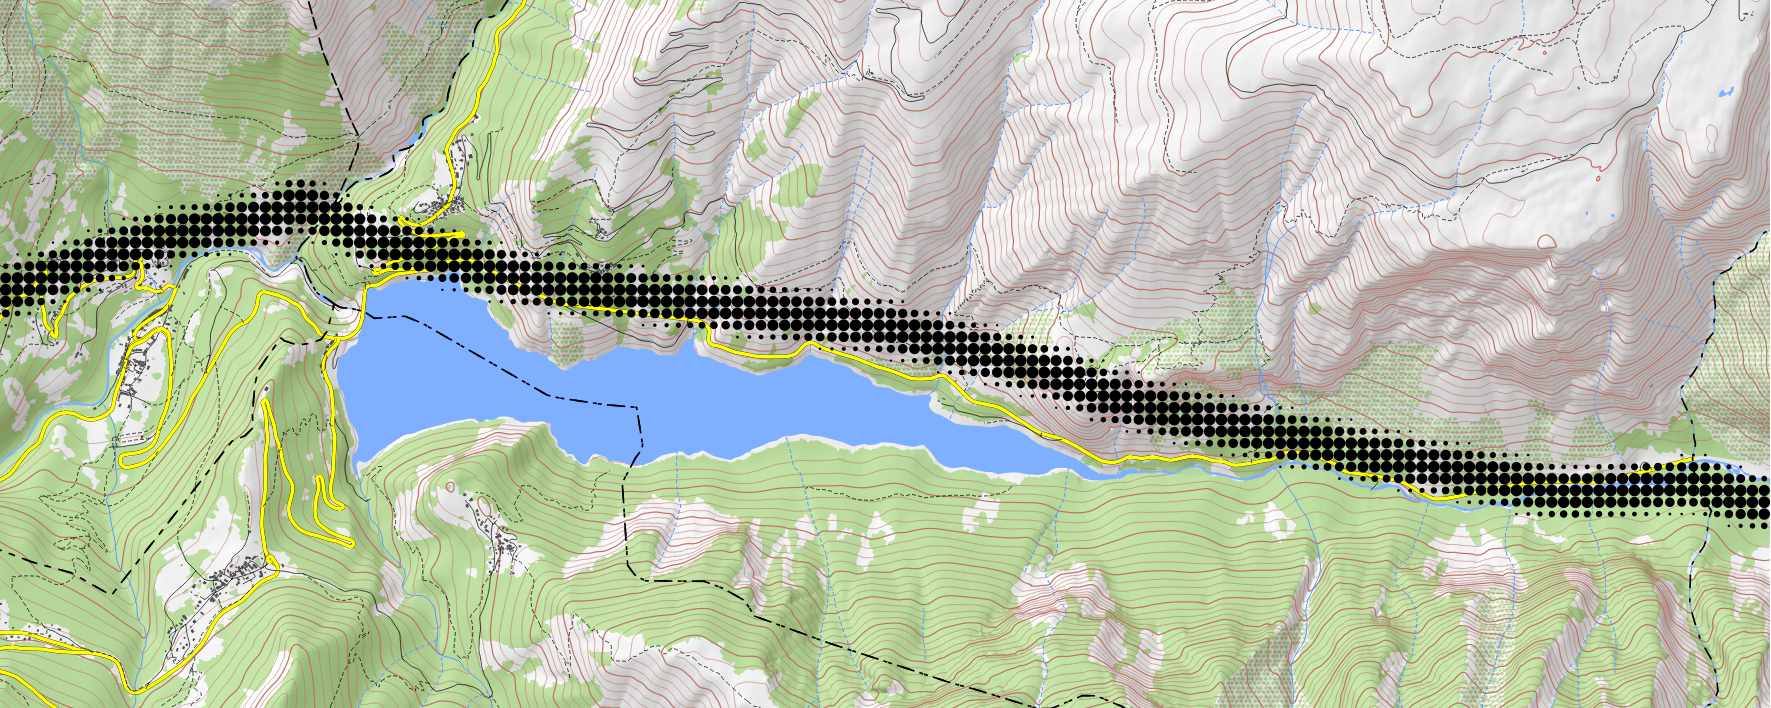
\includegraphics{./figures/Raster_ZLC_DIST_HT.png}};
  % 
  \begin{scope}
    \node (P2) at ([yshift=-.5cm]image.south east) {};
    \node (P1) at ([yshift=-.5cm]image.south west) {};
    % 
    \node (rect) [anchor=north west, minimum width=1cm,minimum
    height=.25cm] at ([yshift=-.25cm]P1) {}; \path[draw=RdBu-9-1, line
    width=.4mm](rect.west) --([xshift=-1ex]rect.south) -- ([xshift=1ex]rect.north)
    -- (rect.east);
    \node[anchor=west, font=\tiny\vphantom{Ag}, text width = 4cm] at
    ([xshift=1ex]rect.east) {Ligne électrique utilisée comme
      \emph{objet de référence}};

    \foreach \x [evaluate=\xshift using \x/10, evaluate=\rad using (\x * .0004) + .01] in {0,...,100}
    {
      \draw[fill=black,draw=none, below] ([xshift=\xshift cm, yshift=-1.5cm]P1) circle [radius=\rad cm];
    }
    % 
    \path(P1 |- 0cm,-2cm) --++ (10,0)
    node[et,pos=0] {0}
    node[et,pos=.1] {0,1}
    node[et,pos=.2] {0,2}
    node[et,pos=.3] {0,3}
    node[et,pos=.4] {0,4}
    node[et,pos=.65] {0,65}
    node[et,pos=1] {1};
    % Échelle
    \draw[-] (P2 |- -1cm,-1cm) --++ (-1,0) node[et,pos=.5] {\SI{500}{\meter}};
    % Légende détaillée
    \path (P1) -- (P2) node[pos=.5, yshift=-2cm] {\tiny Pour la légende détaillée du fond topographique voir \autoref{anx:topo_leg}. Sources: BD TOPO 2018, BD ALTI 2018.}; 
  \end{scope}
\end{tikzpicture}
  \caption{Mon beau raster}
  \label{fig:ZLC_DIST_HT}
\end{carte}


\begin{carte}
  \centering
  \begin{tikzpicture}
  \tikzset{et/.style={above,font=\footnotesize\vphantom{Ag}}}
  %
  \node[inner sep=0pt, anchor=south west] (image) at (0,0){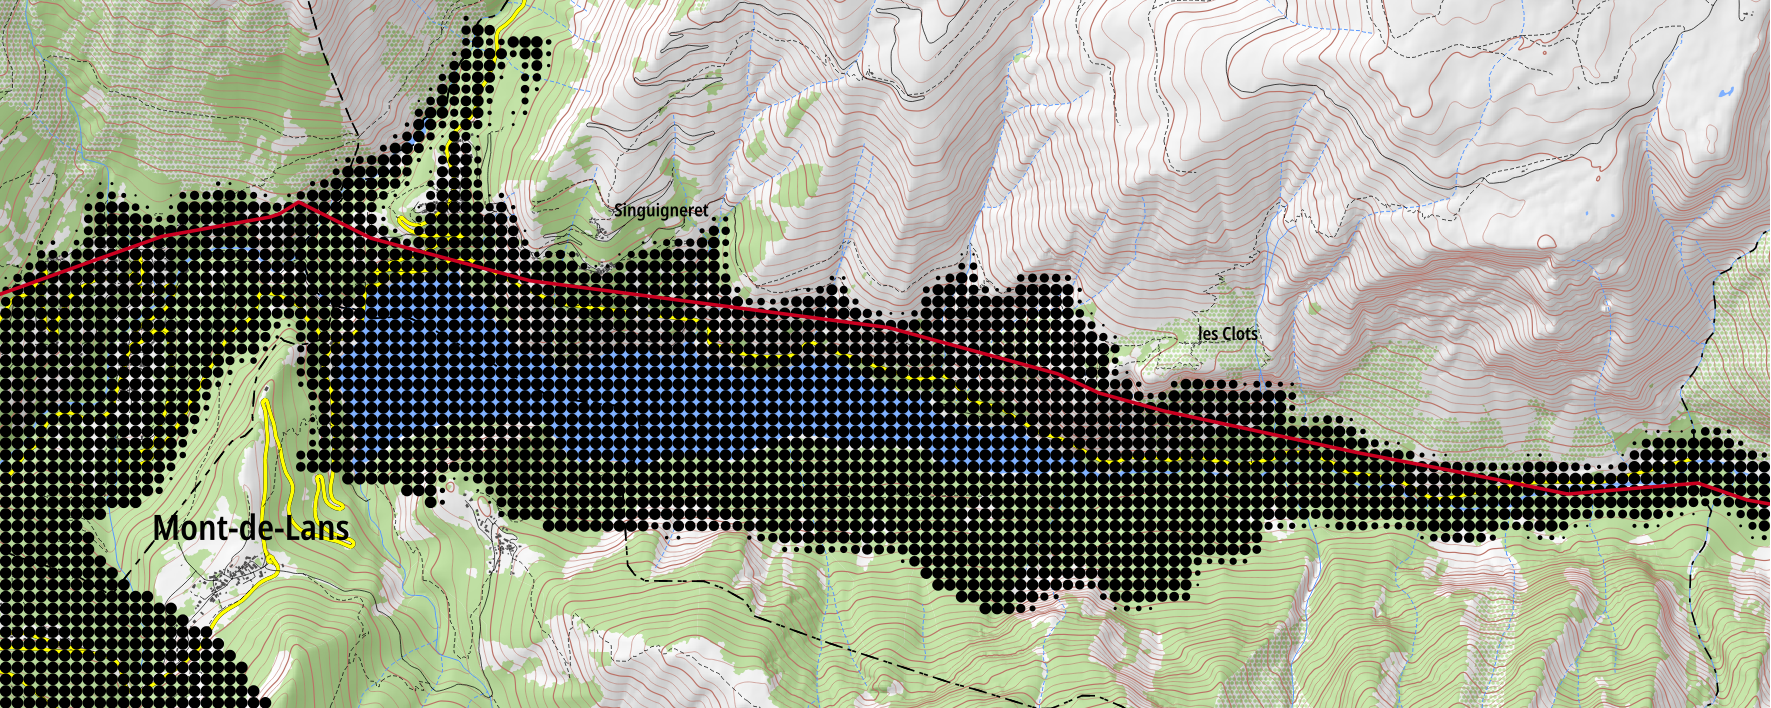
\includegraphics{./figures/Raster_ZLC_ALTINF_HT.png}};
  %
  \begin{scope}
    \node (P2) at ([yshift=-.5cm]image.south east) {};
    \node (P1) at ([yshift=-.5cm]image.south west) {};
    %
    \node (rect) [anchor=north west, minimum width=1cm,minimum
    height=.25cm] at ([yshift=-.25cm]P1) {}; \path[draw=RdBu-9-1, line
    width=.4mm](rect.west) --([xshift=-1ex]rect.south) -- ([xshift=1ex]rect.north)
    -- (rect.east);
    \node[anchor=west, font=\tiny\vphantom{Ag}, text width = 4cm] at
    ([xshift=1ex]rect.east) {Ligne électrique utilisée comme
      \emph{objet de référence}};

    \foreach \x [evaluate=\xshift using \x/10, evaluate=\rad using (\x * .0004) + .01] in {0,...,100}
    {
      \draw[fill=black,draw=none, below] ([xshift=\xshift cm, yshift=-1.5cm]P1) circle [radius=\rad cm];
    }
    % 
    \path(P1 |- 0cm,-2cm) --++ (10,0)
    node[et,pos=0] {0}
    node[et,pos=.1] {0,1}
    node[et,pos=.2] {0,2}
    node[et,pos=.3] {0,3}
    node[et,pos=.4] {0,4}
    node[et,pos=.65] {0,65}
    node[et,pos=1] {1};
    % Échelle
    \draw[-] (P2 |- -1cm,-1cm) --++ (-1,0) node[et,pos=.5] {\SI{500}{\meter}};
    % Légende détaillée
    \path (P1) -- (P2) node[pos=.5, yshift=-2cm] {\tiny Pour la légende détaillée du fond topographique voir \autoref{anx:topo_leg}. Sources: BD TOPO 2018, BD ALTI 2018.}; 
  \end{scope}
\end{tikzpicture}
  \caption{Mon très beau raster}
  \label{fig:ZLC_ALTINF_HT}
\end{carte}

La \emph{zone de localisation probable} correspondant à l'ensemble des
positions situées \emph{à proximité} et à une \emph{altitude
  inférieure} de la ligne à haute-tension est construite en
intersectant les deux \emph{zones de localisation compatibles}
calculées (cartes \ref{fig:ZLC_DIST_HT} et
\ref{fig:ZLC_ALTINF_HT}). Pour cet exemple nous avons utilisé les
opérateurs de \textcite{Zadeh1965}.
% 
La \emph{zone de localisation probable} résultant de cette opération
(\ref{fig:ZLP_SOUS_HT}) est visuellement très similaire à son
équivalent résultant de la méthode par \emph{alpha-cuts.}

\begin{carte}
  \centering
  \begin{tikzpicture}
  \tikzset{et/.style={above,font=\footnotesize\vphantom{Ag}}}
  % 
  \node[inner sep=0pt, anchor=south west] (image) at (0,0){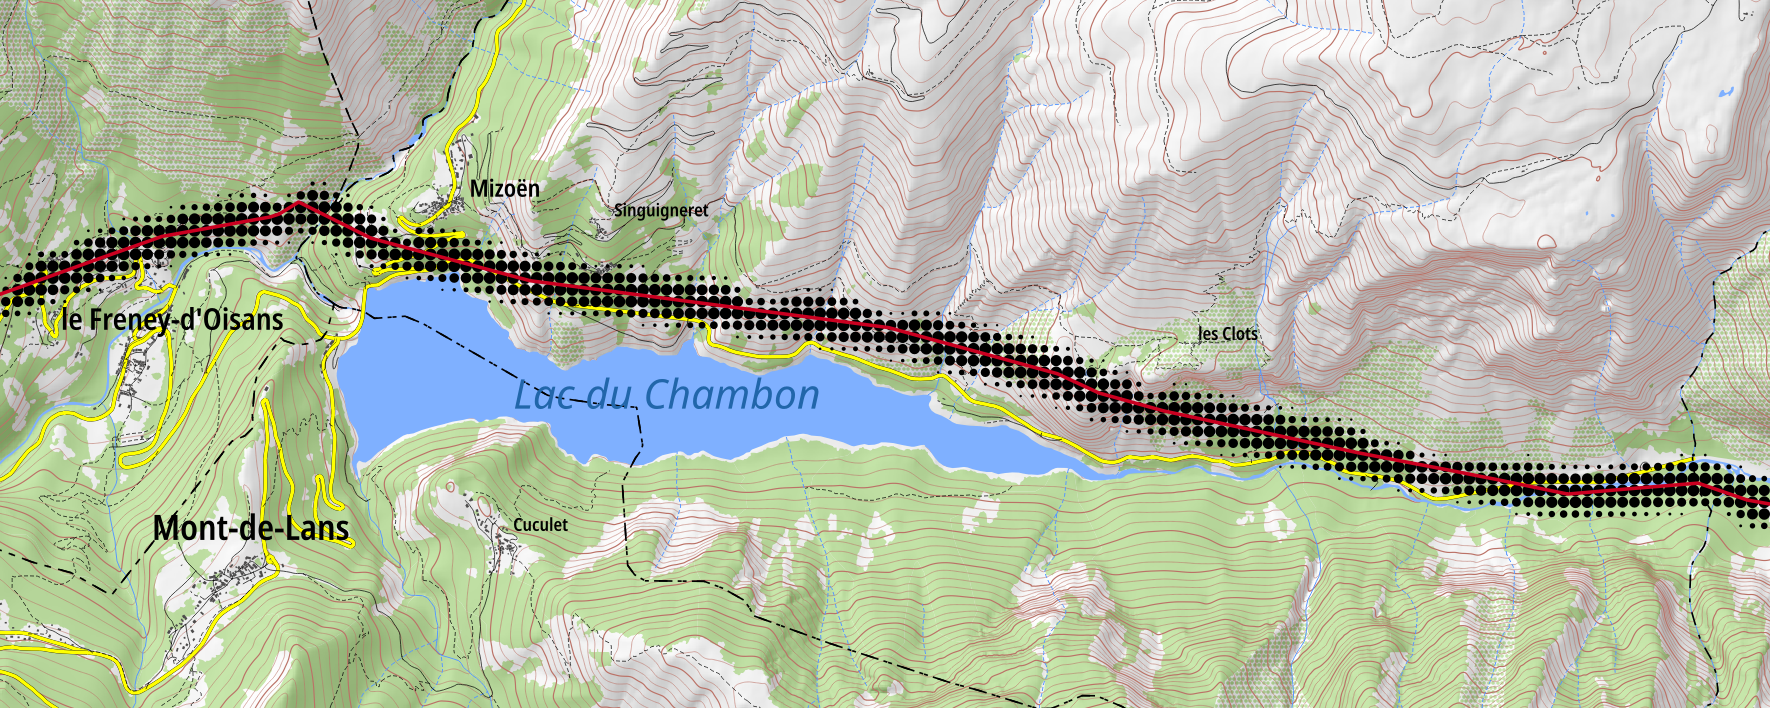
\includegraphics{./figures/Raster_ZLP_SOUS_HT.png}};
  % 
  \begin{scope}
    \node (P2) at ([yshift=-.5cm]image.south east) {};
    \node (P1) at ([yshift=-.5cm]image.south west) {};
    % 
    \node (rect) [anchor=north west, minimum width=1cm,minimum
    height=.25cm] at ([yshift=-.25cm]P1) {}; \path[draw=RdBu-9-1, line
    width=.4mm](rect.west) --([xshift=-1ex]rect.south) -- ([xshift=1ex]rect.north)
    -- (rect.east);
    \node[anchor=west, font=\tiny\vphantom{Ag}, text width = 4cm] at
    ([xshift=1ex]rect.east) {Ligne électrique utilisée comme
      \emph{objet de référence}};

    \foreach \x [evaluate=\xshift using \x/10, evaluate=\rad using (\x * .0004) + .01] in {0,...,100}
    {
      \draw[fill=black,draw=none, below] ([xshift=\xshift cm, yshift=-1.5cm]P1) circle [radius=\rad cm];
    }
    % 
    \path(P1 |- 0cm,-2cm) --++ (10,0)
    node[et,pos=0] {0}
    node[et,pos=.1] {0,1}
    node[et,pos=.2] {0,2}
    node[et,pos=.3] {0,3}
    node[et,pos=.4] {0,4}
    node[et,pos=.65] {0,65}
    node[et,pos=1] {1};
    % Échelle
    \draw[-] (P2 |- -1cm,-1cm) --++ (-1,0) node[et,pos=.5] {\SI{500}{\meter}};
    % Légende détaillée
    \path (P1) -- (P2) node[pos=.5, yshift=-2cm] {\tiny Pour la légende détaillée du fond topographique voir \autoref{anx:topo_leg}. Sources: BD TOPO 2018, BD ALTI 2018.}; 
  \end{scope}
\end{tikzpicture}
  \caption{Mon très très beau raster}
  \label{fig:ZLP_SOUS_HT}
\end{carte}


\subsection{Modélisation par \emph{Alpha-cuts}}

L'implémentation par \emph{alpha-cuts} basée sur l'approche utilisée
par \textcite{Runz2008a,Zoghlami2016}.


\tdi{Revenir un peu sur les alpha-cuts et le lac}

Nécessité d'utiliser CGAL \autocite{CGAL2019}.

\tdi{acuts et intersecions}

\missingfigure{Illustration modélisation concrète par alpha-cuts}


\subsection{Comparaison des approches et choix approche raster}

\paragraph{Comparaison des approches}

\tdi{Difficulté de mise en place}

Au moment de la sélection d'une méthode de modélisation nous avons
estimé que le développement d'une méthode utilisant des vecteurs
serait bien plus coutueuses. Sur ce point nous avons préféré les
rasters. De plus il a été bc plus difficile d'aboutir à une
modélisation vectorielle permettant la comparaison (citer RIG).

\tdi{Difficulté d'extension}

Il semble plus difficile de développer des méthodes de spatialisation
très différentes en vecteur qu'en raster.

Il est également plus compliqué de tester de nouveaux couples
d'opérateurs flous en vecteur.

\tdi{Tendance à la fragmentation des alpha-cuts}

\tdi{Temps de calcul}

% Critère moyennement pertinent
Le critère du temps de calcul n'est pas fondamental pour ce
travail. Toutefois il nous semble pertinent de préciser que les deux
méthodes différent sur ce point.

Avantage raster si le nombre de cellules n'est pas trop
important. Mais le temps de calcul augmente rapidement. L'approche
vecteur est moins rapide mais le code est moins (et plus
difficilement) optimisé. Le résultat est assez mitigé.

\tdi{Volume des données}

Avantage vecteur. Le raster tend à prendre beaucoup de place, encore
plus si l'on souhaite stoquer les objets de référence en raster ou
sauvegarder des résutlats intermédiaires.

\tdi{Qualité de la modélisation}

Comparable, l'article de la RIG n'a pas permis de mettre en évidence
des différences notables. Par construction l'approche vectorielle est
plus précise, mais sa précision dépend aussi des données (MNT pour
l'altitude). À l'échelle du pixel les résultats sont comparables.

\tdi{OK pour les deux: Stabilité du modèle ? (par exemple si l'on fait
  des intersection avec le modèle egg-yolk on doit choisir ce qu'est
  le jaune. C'est l'intersection des jaunes ? ou il suffit qu'il y a
  ait un jaune?  est-ce qu'il faut introduire des valeurs
  intermédiaires (gris, lorsqu'on intersecte jaune et blanc) -> mais
  dans ce cas on sort du egg yolk, le modèle n'est pas stable
  alors). Le résultat doit pouvoir s'exprimer avec la même
  modélisation sans perte de sémantique et de finesse de
  modélisation.}


\paragraph{Choix du raster}


La comparaison de ces deux implémentations de la \emph{théorie des
  sous-ensembles flous} nous a conduit à adopter une démarche fondée sur
l'utilisation de rasters.

\tdi{Plus facile à développer}

\tdi{Plus facile à étendre}

\tdi{Plus rapide d'arriver à spatialiser -> possibilité de travailler
  sur plus d'alertes}

Le premier avantage de cette implémentation est d'ordre technique. Si
cette approche a tendance à être moins performante et plus
consommatrice de ressources informatiques, elle offre en retour
l'avantage d'être plus facile à mettre en place et à étendre. Ainsi,
le choix d'une approche raster nous permet de développer plus
rapidement une méthode fonctionnelle et donc de pouvoir nous
concentrer sur la spatialisation de plus d'alertes et non sur des
aspects plus techniques.

\tdi{Plus facile à utiliser (pas de fragmentation)}

Mais l'approche raster se distingue également par ces caractéristiques
XXXX. En réduisant toutes les opérations inter-\emph{zones de
  localisation} à des opérations arithmétiques composantes à
composantes, l'approche raster permet de conserver une certaines
stabilité du résultat, contrairement à l'approche par
\emph{alpha-cuts.}


Le choix d'utiliser une modélisation basée sur la \emph{théorie des
  sous-ensembles flous} et implémentée à l'aide de raster à des
conséquences théoriques et pratiques.

\tdi{Nécessité de choix des opérateurs flous}

Les différentes opérations inter-\emph{zones de localisation} peuvent
être réalisée avec différents opérateurs flous.

\tdi{Nécessité de définir une résolution}

De plus, l'utilisation de rasters pose un autre questionnement, celui
de la définition d'une résolution, dont dépendra la finesse, le poids
et la rapidité de construction des \emph{zones de localisation.}

%%% Local Variables:
%%% mode: latex
%%% TeX-master: "../../../../main"
%%% End:
